%%%%%%%%%%%%%%%%%%%%%%%%%%%%%%%%%%%%%%%%%
% Focus Beamer Presentation
% LaTeX Template
% Version 1.0 (8/8/18)
%
% This template has been downloaded from:
% http://www.LaTeXTemplates.com
%
% Original author:
% Pasquale Africa (https://github.com/elauksap/focus-beamertheme) with modifications by 
% Vel (vel@LaTeXTemplates.com)
%
% Template license:
% GNU GPL v3.0 License
%
% Important note:
% The bibliography/references need to be compiled with BibTeX.
%
%%%%%%%%%%%%%%%%%%%%%%%%%%%%%%%%%%%%%%%%%
% https://www.latextemplates.com/template/focus-presentation

%----------------------------------------------------------------------------------------
% PACKAGES AND OTHER DOCUMENT CONFIGURATIONS
%----------------------------------------------------------------------------------------

\documentclass{beamer}
\usepackage[ngerman]{babel}

\usetheme{focus} % Use the Focus theme supplied with the template
% Add option [numbering=none] to disable the footer progress bar
% Add option [numbering=fullbar] to show the footer progress bar as always full with a slide count

% Uncomment to enable the ice-blue theme
% \definecolor{main}{RGB}{92, 138, 168}
% \definecolor{background}{RGB}{240, 247, 255}

%------------------------------------------------

\usepackage{booktabs} % Required for better table rules

%----------------------------------------------------------------------------------------
% TITLE SLIDE
%----------------------------------------------------------------------------------------

\title{Optische Fouriertransformation}

\subtitle{MathSem 2023}

\author{Marco Niederberger \texorpdfstring{\\}{} Yanick Schoch}

\titlegraphic{\includegraphics[scale=0.5]{../../SeminarHarmonischeAnalysis/buch/papers/opt/images/jamesWebb_cropped_publicDomain.png}} % Optional title page image, comment this line to remove it

\institute{OST - Ostschweizer Fachhochschule}

\date{08. Mai 2023}

%------------------------------------------------

\begin{document}

%------------------------------------------------

%% Steady screen for start
{
\setbeamercolor{background canvas}{bg=black}
\begin{frame}[plain]
    % \makebox[\pdfpagewidth]{\includegraphics[height=\paperheight]{../../SeminarHarmonischeAnalysis/buch/papers/opt/images/jamesWebb_publicDomain.png}}
    \begin{tikzpicture}[overlay, remember picture]
        % \fill[color=black] (current page.north west) rectangle (current page.south east);
        \node[inner sep=0pt] at (current page.center)
        {\includegraphics[height=\pdfpageheight]{../../SeminarHarmonischeAnalysis/buch/papers/opt/images/jamesWebb_publicDomain.png}};
    \end{tikzpicture}
\end{frame}
}

\begin{frame}
    \maketitle % Automatically created using the information in the commands above
\end{frame}

% Overview
\begin{frame}{Heutige Ziele}
    \begin{itemize}
        \item Beugung im Allgemeinen
        \item Herleitung des Beugungsintegrals
        \item Versuch
        \item Anwendungen
    \end{itemize}
\end{frame}

%----------------------------------------------------------------------------------------
% SECTION 1
%----------------------------------------------------------------------------------------

\section{Grundlagen} % Section title slide, unnumbered

%------------------------------------------------

\begin{frame}{Grundlagen - Beugung von Wellen}
    \centering
    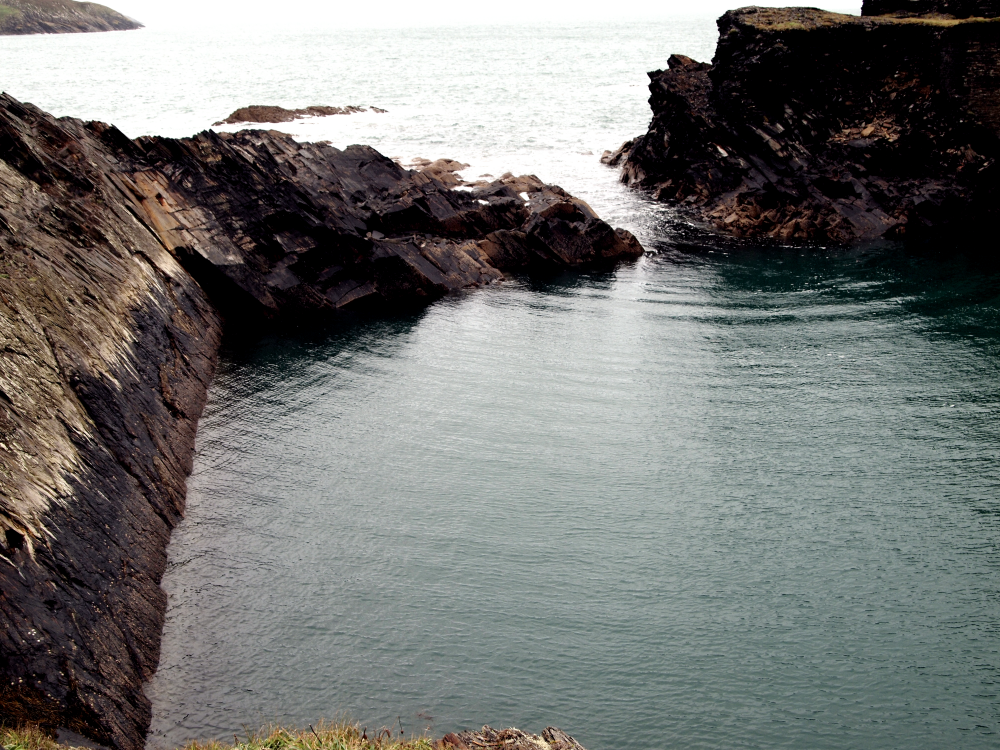
\includegraphics[width=0.9\linewidth]{images/beugung_von_wasserwellen.png}
\end{frame}

\begin{frame}{Grundlagen - Prinzip von Huygens}
    \includegraphics[width=\linewidth]{../../SeminarHarmonischeAnalysis/buch/papers/opt/images/huygens.pdf}
\end{frame}

\begin{frame}{Grundlagen - Wellendarstellung}
    \begin{center}
        \includegraphics[width=0.7\linewidth]{../../SeminarHarmonischeAnalysis/buch/papers/opt/images/welle.pdf}
    \end{center}
    \begin{equation*}
        \zeta(x, t)
        =
        \zeta_0 \cdot e^{j(\omega t - \vec{k}\cdot\vec{x})}
    \end{equation*}
    \begin{equation*}
        k
        =
        \frac{\omega}{u}
        =
        \frac{2 \pi}{\lambda}
    \end{equation*}
\end{frame}

\begin{frame}{Grundlagen - Maxwell}
    \begin{align*}
        \oint_{S=\partial V} \varepsilon\vec{E} \cdot\, d\vec{S}
        &=
        \int_{V}\rho\, dV
        \\
        \int_{0}^{a}\int_{0}^{2\pi} \varepsilon E\cdot 1 \cdot r\, d\varphi dl
        &=
        Q
        \\
        2\pi ra\varepsilon E
        &=
        Q
    \end{align*}
    \begin{equation*}
        E(r)
        =
        \frac{Q}{2\pi\varepsilon a} \cdot \frac{1}{r}
        =
        C \cdot \frac{1}{r}
    \end{equation*}
\end{frame}

\begin{frame}{Grundlagen - Beugungsintegral}
    \begin{center}
        \includegraphics[width=0.7\linewidth]{../../SeminarHarmonischeAnalysis/buch/papers/opt/images/derivation.pdf}
    \end{center}
    % \begin{equation*}
    %     E(y_p, t)
    %     =
    %     C\zeta_0 \cdot \int_{-\infty}^{\infty}f(y)\cdot\frac{e^{j(\omega t - \vec{k}\cdot\vec{r})}}{r} \,dy
    % \end{equation*}
    \begin{equation}
        dE
        =
        E(r) \cdot \zeta(r, t) \cdot dy
        =
        \frac{C}{r} \cdot \zeta_0 \cdot e^{j(\omega t - \vec{k}\cdot\vec{r})} \cdot dy
    \end{equation}
\end{frame}

\section{Versuch}

\begin{frame}{Versuch - Laser aufweiten}
    \centering
    \includegraphics[width = 0.8\textwidth]{../../SeminarHarmonischeAnalysis/buch/papers/opt/images/laserAufweiten.pdf}
\end{frame}

\begin{frame}{Versuch - 4f Aufbau}
    \includegraphics[width = \textwidth]{../../SeminarHarmonischeAnalysis/buch/papers/opt/images/4fAufbau.pdf}
\end{frame}

\section{Anwendungen}

\begin{frame}{Anwendungen - Pattern matching}
    \begin{itemize}
        \item Filterung mit dem gewünschten Spektrum
        \item Simple Helligkeitsdetektion
    \end{itemize}
\end{frame}

\begin{frame}{Anwendungen - Diffractive deep neural network}
    \begin{itemize}
        \item Handschrifterkennung mit Beugung
        \item Fünf Beugungsebenen
        \item Zehn Detektoren
    \end{itemize}
\end{frame}

\begin{frame}{Anwendungen - Diffractive deep neural network}
    \centering
    \includegraphics[width = 1\textwidth]{../../SeminarHarmonischeAnalysis/buch/papers/opt/images/handwriting_xing.png}
    Xing et al. \cite{opt:Lin.2018}
\end{frame}

\begin{frame}{Anwendungen - Diffractive deep neural network}
    \begin{columns}
        \column{0.5\textwidth}
        \includegraphics[width = 1\textwidth]{../../SeminarHarmonischeAnalysis/buch/papers/opt/images/handwriting_5_input_xing.png}
        Input
        \column{0.5\textwidth}
        \includegraphics[width = 1\textwidth]{../../SeminarHarmonischeAnalysis/buch/papers/opt/images/handwriting_5_output_xing.png}
        Output
    \end{columns}
\end{frame}

%% End
\begin{frame}{Ziel erreicht?}
    \begin{itemize}
        \item Was ist Beugung?
        \item Wie kommt die Fouriertransformation zustande?
        \item Für was ist das nützlich?
    \end{itemize}
\end{frame}

%----------------------------------------------------------------------------------------
% CLOSING/SUPPLEMENTARY SLIDES
%----------------------------------------------------------------------------------------

\appendix

\begin{frame}{Appendix - Referenzen}
    \nocite{*} % Display all references regardless of if they were cited
    \bibliography{example.bib}
    \bibliographystyle{plain}
\end{frame}

\begin{frame}{Appendix - Bildquellen}
    Beugung von Wasserwellen: \\
    \url{https://www.rhetos.de/html/lex/beugung_von_wasserwellen.htm}
\end{frame}
%------------------------------------------------

\begin{frame}{Appendix - Hintergrundinformationen}
    \begin{itemize}
        \item \LaTeX{} Präsentation mit dem Theme \emph{Focus}
    \end{itemize}

\end{frame}

\begin{frame}{Appendix - Wellenlängen}
    \begin{table}
        \centering % Centre the table on the slide
        \begin{tabular}{l c}
            \toprule
            Lichtfarbe & Wellenlänge in nm \\
            \toprule
            Violett    & $380 - 420$       \\
            Blau       & $420 - 490$       \\
            Grün       & $490 - 575$       \\
            Gelb       & $575 - 585$       \\
            Orange     & $585 - 650$       \\
            Rot        & $650 - 780$       \\
            \bottomrule
        \end{tabular}
        \caption{Wellenlänge von sichtbarem Licht}
    \end{table}
\end{frame}

%----------------------------------------------------------------------------------------

\end{document}
